\subsubsection{从特征映射到核展开}
\label{sec:classic-overview-kernel-trick}

二分类模型在输入空间中划出一条边界：边界一侧预测正类，另一侧预测负类。原始坐标的加权和只能产生直线（二维时）或超平面（高维时）边界。若两类样本恰好能被一条直线分开，线性模型足够；但类别也可能按“到原点的距离是否小于 $1$”来区分，这时正类挤在单位圆内、负类散在圆外，任何一条直线都无法把整个圆内区域与圆外区域干净分开——无论直线画在哪里，圆的这一侧和那一侧都会同时出现两类点。

判断一个点在圆内还是圆外，需要的是半径平方 $x_1^2+x_2^2$。线性模型不认识平方项，但我们可以替它造出来：把 $x_1^2+x_2^2$ 整体当作一个新特征，再继续使用熟悉的线性得分。也就是说，不是让分类器在原坐标里硬画曲线，而是先把数据搬到一组新坐标，使在新坐标里分界重新变成直线。

图\ref{fig:classification-kernel-map}采用映射$\bm{\phi}(\bm{x})=(x_1,x_1^2+x_2^2)^{\top}$，将圆$x_1^2+x_2^2=1$对应到直线$\phi_2=1$。得分$g(\bm{x})=1-x_1^2-x_2^2$于是写成$g(\bm{x})=(0,-1)\bm{\phi}(\bm{x})+1$：对原坐标非线性，对新特征却是线性的。样本类别保持不变，改变的只是描述它们的坐标；图中边界是教学构造，并非由数据训练得到的最优分类边界。

\begin{figure}[htbp]
  \centering
  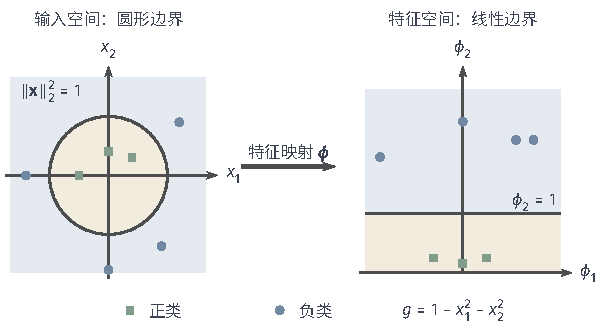
\includegraphics[width=103.166mm]{figures/07-classic-models/00-shared/tikz/classification-kernel-map/figure.pdf}
  \caption{非线性边界在特征映射前后的对应，两个面板的坐标均无量纲。正类方点为$(-0.5,0)$、$(0,0.4)$、$(0.4,0.3)$，负类圆点为$(-1.4,0)$、$(0,-1.6)$、$(1.2,0.9)$、$(0.9,-1.2)$。右图逐点使用$\phi_1=x_1$、$\phi_2=x_1^2+x_2^2$；水平线$\phi_2=1$对应左图半径为1的圆。数据与边界均为教学构造。}
  \label{fig:classification-kernel-map}
\end{figure}

圆形例子只需计算一个新特征，成本可以忽略。但若为了描述更复杂的弯曲关系而加入大量平方项、两两交互项甚至更高次项，显式列出所有新坐标就可能非常昂贵：仅二次映射，$d$ 个原变量就要产生约 $d^2/2$ 个新坐标，次数再升高数量还会快速增长；计算、存储和后续求解都要承担这份开销。于是出现一个关键问题：能不能在不真正写出、也不保存这些新坐标的情况下，照样完成计算？

\emph{从“只需内积”到核展开。}要回答这个问题，先检查线性算法到底怎样使用特征。给定$n$个训练输入$\bm x_1,\ldots,\bm x_n$，设$\bm\phi$将输入映射到带内积的特征空间$\mathcal H$，在那里使用线性得分$\langle\bm w,\bm\phi(\bm x)\rangle+b$。

在一类常见的训练问题里，训练损失只依赖各训练点的得分，而惩罚是参数范数的非减函数。把$\mathcal H$中的任意参数向量分解为“训练特征张成空间内的部分”与“正交于该空间的部分”：正交部分与每个训练特征的内积都是零，把它加到 $\bm w$ 上不会改变任何训练点的得分，却只会增大参数范数，从而增大惩罚。删去这一正交部分，训练得分不变、惩罚不增，因此若最优解存在，总能在这 $n$ 个训练特征张成的空间里找到它（张成空间＝这些特征向量线性组合能够到达的全部方向），即存在一组系数 $a_i$ 使
\begin{equation}
  \bm w=\sum_{i=1}^n a_i\bm\phi(\bm x_i).
  \label{eq:classic-overview-weight-expansion}
\end{equation}
这一展开只说明“有解时解可取在训练特征张成内”，并不单独证明解存在或唯一；存在性与唯一性仍由具体学习目标决定。

把这一展开代回线性得分，内积的线性性质允许把求和提到内积外面：
\begin{equation}
  \begin{aligned}
    K(\bm x,\bm z)
      &=\langle\bm\phi(\bm x),\bm\phi(\bm z)\rangle_{\mathcal H},\\
    f(\bm x)&=\sum_{i=1}^n a_iK(\bm x_i,\bm x)+b.
  \end{aligned}
  \label{eq:classic-overview-kernel}
\end{equation}
这里三者职责不同：核 $K$ 只给出两个输入映射后的特征内积，样本系数 $a_i$ 由具体学习目标确定，截距 $b$ 处理特征均值未被零化的整体偏移。预测时只需逐个计算新输入与训练输入的核值，既不必写出映射后的坐标，也不必保存高维的 $\bm w$。这种用核值完成特征内积计算的办法称为\term{核技巧}（kernel trick）；当$K$对原输入非线性时，特征空间中的线性得分也能描述原空间中的非线性关系，而显式特征展开这一步被完全绕过。

注意，式~\eqref{eq:classic-overview-kernel}只保证“预测”能改写为核值计算；要连训练也一起省去显式特征，训练问题本身也必须只通过核值使用特征。例如训练损失只使用各训练点的得分，并以正系数惩罚参数范数平方时，前面关于正交部分的论证正好适用：正交部分不改变训练得分却增加惩罚，最优解自然落在训练特征张成的空间内，于是整个训练都可用上述有限展开完成。具体到支持向量机，这一对偶形式将在分类章推导。核决定的是特征表示，分类、回归等任务仍由各自的损失和约束确定学习目标。

\subsubsection{合法核、常用核与超参数}
\label{sec:classic-overview-kernel-validity}
\label{sec:classic-overview-common-kernels}

\emph{什么样的函数才能充当核。}先注意这里说的“核”是特征内积的代称，与回归章局部加权里“按距离给记录加权重”的核只是同名：那个距离权重核只决定邻域内的加权平均，并不对应某个特征空间。核函数要能真正写成某个特征映射的内积，即 $K(\bm x,\bm z)=\langle\bm\phi(\bm x),\bm\phi(\bm z)\rangle_{\mathcal H}$。

\emph{充要条件。}一个对称函数 $K$ 能充当核，充要条件是对任意有限个输入 $\bm x_1,\ldots,\bm x_m$ 和任意实系数 $c_1,\ldots,c_m$，二次型 $\sum_{i,j=1}^m c_ic_jK(\bm x_i,\bm x_j)\ge0$；把核值两两排成 Gram 矩阵后，这就是矩阵半正定。该条件允许 Gram 矩阵奇异（存在非零系数使二次型恰为零），不额外要求可逆。反过来，满足对称与有限半正定条件的函数必对应某个特征映射：由它出发可以造出以 $K$ 为再生核的函数空间，所以不必真的写出 $\bm\phi$，上述条件本身就是“存在某个 $\bm\phi$”的充要依据。这两条结论的严格表述可参考\BookChapterRef{subsubsec:point-evaluation}{卷一《数学准备：计算、分析与几何》“函数空间”章中关于正定核的段落}；连续核在紧输入域上沿有限测度的谱展开还需要连续性与定义域等附加条件（见该章\BookSectionRef{subsubsec:compact-spectrum-mercer}{第~\ref{subsubsec:compact-spectrum-mercer}节}的Mercer展开），不能误列为所有合法核的必要条件。

合法性检查的是“所有实系数形成的二次型是否非负”，要避免几种常见误解。它不是检查每个核值本身是否非负——合法核在不相似的两点上完全可以取负值（例如未加常数的线性核）。它也不是凭“看起来像相似性”就能成立。只检查某一份训练集上的矩阵，只能确认这一组输入合法；新输入还必须落在核已确认合法的定义域内。此外，合法核只提供“它确实对应某个特征内积”的依据，并不保证这个特征表示适合当前任务，也不保证对应的学习目标容易求解——合法性与有效性是两件事。

对$\bm x,\bm z\in\mathbb R^d$，选择不同的核，等于暗中选择了不同的特征空间和特征关系。表\ref{tab:classic-overview-common-kernels}列出常见形式及条件；核尺度记为$\beta$，多项式次数记为$p$，与输入维数$d$区分。

\begin{table}[htbp]
  \centering
  \small
  \begin{tabularx}{\linewidth}{@{}>{\RaggedRight\arraybackslash}p{18mm}>{\RaggedRight\arraybackslash}X>{\RaggedRight\arraybackslash}p{27mm}@{}}
    \toprule
    名称 & $K(\bm{x},\bm{z})$ & 参数与正定性\\
    \midrule
    线性核 & $\bm{x}^{\top}\bm{z}$ & 半正定\\
    多项式核 & $(\beta\bm{x}^{\top}\bm{z}+r)^p$ & $\beta,r\ge0$，正整数$p$\\
    高斯RBF核 & $\exp(-\beta\lVert\bm{x}-\bm{z}\rVert_2^2)$ & $\beta>0$，半正定\\
    Laplacian核 & $\exp(-\beta\lVert\bm{x}-\bm{z}\rVert_1)$ & $\beta>0$，半正定\\
    Sigmoid形式 & $\tanh(\beta\bm{x}^{\top}\bm{z}+r)$ & 一般不保证半正定\\
    \bottomrule
  \end{tabularx}
  \caption{常用核函数与合法性条件。这里的“半正定”要求任意有限输入的Gram矩阵半正定；Sigmoid一行列出的是常见相似性形式，使用前仍需针对定义域与参数核验。}
  \label{tab:classic-overview-common-kernels}
\end{table}

\term{线性核}（linear kernel）就是原始特征的内积，不增加任何新特征，对应普通的线性模型，常作为比较基准。\term{多项式核}（polynomial kernel）隐式加入了有限阶的特征交互：把 $(\beta\bm x^\top\bm z+r)^p$ 展开后，各项对应原变量的各次乘积，因此 $p=2$ 时能表达平方项和两两乘积，$p$ 更大时表达更高次的组合。在$\beta>0$时，$r=0$只保留$p$次项，$r>0$则包含从常数项到$p$次项的各阶特征；参数取零时，相应特征块可以消失。核计算省去的是这些坐标的显式展开，完整训练成本仍取决于样本数和学习目标。

\term{高斯径向基核}（Gaussian radial basis function kernel，Gaussian RBF kernel）不看方向上的投影，而按两点的欧氏距离衡量局部接近程度：两点重合时核值为 $1$，距离越远核值平滑衰减到 $0$。常将$\beta$写成$1/(2\sigma^2)$，其中$\sigma>0$是距离尺度：$\sigma$ 越大（$\beta$ 越小），核值衰减越慢，一个点能影响的范围越宽；$\sigma$ 越小（$\beta$ 越大），作用范围越局部。它对应的特征空间是无限维的，因而能表达相当灵活的非线性关系，但作用范围是否合适仍需结合数据判断，不能仅凭“能拟合弯曲边界”就断定新样本误差更小。

\term{Laplacian核}（Laplacian kernel）形式相近，只是把欧氏距离换成$L^1$距离，即各坐标绝对差之和；$L^1$距离沿坐标轴方向变化，改变了衡量“接近”的几何，对某些坐标轴对齐的结构更敏感。

常称为\term{Sigmoid核}（sigmoid kernel）的形式把内积送入双曲正切函数，在神经网络兴起后常被使用，但它一般不保证正定核所需的半正定性；只取正参数也不足以替代对定义域和参数取值的合法性核验，使用前必须单独检查或改用其他核。核尺度、多项式次数、正则化强度等在一次拟合前固定的配置，可以用验证数据在训练内选择；配置确定后，还要用未参与选择的新数据评价预测误差，不能把选择配置时用过的数据再当作最终评价依据。
